%!TEX root =../../thesis-ex.tex

\section{Definition of Decision Making and Decision Support Systems}

In this thesis, we consider both user decision and decision making as their most general sense possible. Decision making is the activity for a user to interact with systems on her device, where the user have to choose from a set of options, and the selection is related to the users' personal benefit, e.g., money, security, or a significant amount of time. 

Under this definition, most activities for the user to interact with an information system (i.e., search engine or recommender system) are within the scope of decision making. For example, when a user needs to make selection for which paper to read next, or which movie to watch next, it may require a significant amount of time, therefore these activities should also be categorized as decisions. Interactive activities that we do not consider as decisions are tasks where the interactions are fixed and without much uncertainty, e.g., the how-to activities such as how to attach a photo to a Tweet. 

Similarly, we consider decision support systems a general concept. A decision support system is any system that provides information more than the original information and assist users reduce the uncertainty of decision making. As a result, any recommender system (e.g., people who bought this also bought) is a decision support system under our definition, because the suggested items allows users to observe similar items more efficiently which could potentially lead to a purchase decision. A question answering shopping agent is also a decision support system because it helps the users to reduce the uncertainty for a produce. Therefore, the decision support can be in two ways: first, the system initiate the decision support by actively providing information; second, the system support decisions on demand and provide the information specified by the user. 

\section{User Decision Making on Mobile Devices}
\label{ch1:sec2:motiv}

With the prevalence of mobile devices, billions of users rely on mobile devices to fulfill their daily tasks. During interaction with mobile devices, users often need to face the challenge of \emph{making decisions}. That is, choosing between options, where the selection can affect users' personal benefit, e.g., money or security. Today, statistics suggest that more and more user decisions are made on smaller devices, e.g., statistics predict that by 2021, mCommerce will dominate the sales, with more than 53.9\% sales coming from mobile devices~\cite{mcommerce53}.

Decision making is a slow judgment process. Different from fast judgment tasks such as visual object recognition, speech recognition, slow judgment process often involves complicated mental models and user efforts in researching, exploration, learning new knowledge, and comparison. For example, when making shopping decisions for a product that they are unfamiliar with, users usually do not settle down on the first search result right away, but they need to researching information such as the price distribution for that product, what are the most popular name brands, etc, before finalizing the decision. For business decision, it may involve special programming skills such as querying a database. The lack of such knowledge thus creates a gap between user and the optimal decision. 

In general, the knowledge gap can be caused by the following reasons. First, \emph{transparency of the system}. When certain operations of the system cannot be known, from the users' side, it is difficult to make decisions based on the partially available or not available information, one example is security decision making on granting permissions where the user has no access to directly observing how exactly the permissions are being used, another example is AI systems that automatically make decisions for users. Second, \emph{decisions need to be made from a large database}. When decisions need to be made from a large database, it is impossible for the user to go through all the options, therefore even the system supports keywords search, it still possible that the user have missed some options, this problem is amplified if the keywords search function is poorly supported or it is difficult for the user to formulate a good query, one example is clothes search in a shopping website. Third, \emph{making decisions require specialized knowledge}. For example, when querying a database for making business decisions, a data analyst needs to know the grammar of SQL. Without other supports, it would be difficult for the data analyst to perform such queries. 

The knowledge gap for decision making on mobile devices is further amplified. As discussed in Section~\ref{ch1:sec1:background}, mobile user interactions are affected by its screen size, difficulty in typing and difficulty understanding permission requests. With \emph{typing difficulty}, it is more difficult for users to interact with search engines as like in computers. With \emph{smaller screens}, it is also more difficulty for users to navigate through the search results. Also with \emph{difficulty typing and editing}, users face more challenges searching for answers to difficult and technical questions, e.g., questions on coding tasks. Mobile systems also introduces its new decision scenarios, i.e., when requesting security permissions, users often do not understand the purpose behind such requests, for average users, without explanation by the app developers, it is very difficult for them to obtain such knowledge from other places, e.g., Google.

\section{Bridging Knowledge Gap for Decision Making}

One essential way for assisting users' decision making tasks is to suggest external knowledge to users before the decisions need to be made. Such knowledge support systems are often seen in information systems. For example, along with Google search results, the engine often actively suggest related knowledge entries, e.g., if the user searches for a shopping related query, the search engine not only display results that answers the query, but also related knowledge which goes beyond the query itself, e.g., how much a mattress box spring costs (Figure~\ref{ch1:fig2:knowledge1}). Such knowledge may help users make better decisions, e.g., by knowing how much a good box spring cost, users are less likely to pay more money than they need to. 

\begin{figure}[h]
\centering
\subfloat[][``People also ask'' (both desktop and mobile)]{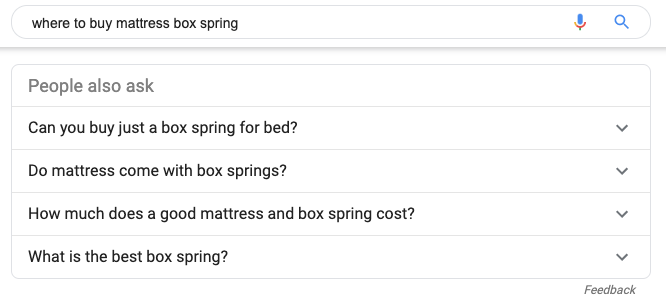
\includegraphics[width=.6\textwidth]{figure/chapter1/knowledge1}\label{ch1:fig2:knowledge1}}\hfill
\subfloat[][``Interesting finds'' (mobile only)]{
\includegraphics[width=.3\textwidth]{figure/chapter1/knowledge3}\label{ch1:fig2:knowledge2}}
\caption{Google actively suggest knowledge entries to help users making decisions}
\end{figure}

On mobile devices, by realizing the knowledge gap, Google has further enhanced the knowledge support. Besides also displaying the knowledge entries as on desktop, Google further enriches the mobile search results, including showing ``interesting finds'' (Figure~\ref{ch1:fig2:knowledge2}). In general, Google's mobile search results is much more diversified than desktop search results. 

Knowledge support is also often seen in clinical decision support systems, where the system helps users to retrieve medical documents, disambiguate difficult medical terms and answer questions~\cite{sankhavara2018biomedical}. 

The general methodology behind knowledge assistance include the follows. First, \emph{retrieval}. If the knowledge entry is a natural language sentence, it can be directly retrieved from a candidate corpus by defining a scoring function. When the suggested knowledge can be directly adopted from the original data, and when the data size is large enough, retrieval has many advantages, including efficiency, good interpretability and low cost. Notably, with retrieval approaches, labeled data can be leveraged but it is not required. For example, retrieval-based question answering is often used in question answering systems. Second, \emph{summarization}. Sometimes the user needs to get a knowledge of the data distribution of the corpus, where summarization could help. For example, histogram summarizes the distributional statistics of the corpus. Topic models summarizes the main content in the documents. Third, \emph{generation}. Different from retrieval, generation can be applied even when the dataset does not contain the answer to the question being answered. 
